\documentclass{article}\usepackage[]{graphicx}\usepackage[]{xcolor}
% maxwidth is the original width if it is less than linewidth
% otherwise use linewidth (to make sure the graphics do not exceed the margin)
\makeatletter
\def\maxwidth{ %
  \ifdim\Gin@nat@width>\linewidth
    \linewidth
  \else
    \Gin@nat@width
  \fi
}
\makeatother

\definecolor{fgcolor}{rgb}{0.345, 0.345, 0.345}
\newcommand{\hlnum}[1]{\textcolor[rgb]{0.686,0.059,0.569}{#1}}%
\newcommand{\hlsng}[1]{\textcolor[rgb]{0.192,0.494,0.8}{#1}}%
\newcommand{\hlcom}[1]{\textcolor[rgb]{0.678,0.584,0.686}{\textit{#1}}}%
\newcommand{\hlopt}[1]{\textcolor[rgb]{0,0,0}{#1}}%
\newcommand{\hldef}[1]{\textcolor[rgb]{0.345,0.345,0.345}{#1}}%
\newcommand{\hlkwa}[1]{\textcolor[rgb]{0.161,0.373,0.58}{\textbf{#1}}}%
\newcommand{\hlkwb}[1]{\textcolor[rgb]{0.69,0.353,0.396}{#1}}%
\newcommand{\hlkwc}[1]{\textcolor[rgb]{0.333,0.667,0.333}{#1}}%
\newcommand{\hlkwd}[1]{\textcolor[rgb]{0.737,0.353,0.396}{\textbf{#1}}}%
\let\hlipl\hlkwb

\usepackage{framed}
\makeatletter
\newenvironment{kframe}{%
 \def\at@end@of@kframe{}%
 \ifinner\ifhmode%
  \def\at@end@of@kframe{\end{minipage}}%
  \begin{minipage}{\columnwidth}%
 \fi\fi%
 \def\FrameCommand##1{\hskip\@totalleftmargin \hskip-\fboxsep
 \colorbox{shadecolor}{##1}\hskip-\fboxsep
     % There is no \\@totalrightmargin, so:
     \hskip-\linewidth \hskip-\@totalleftmargin \hskip\columnwidth}%
 \MakeFramed {\advance\hsize-\width
   \@totalleftmargin\z@ \linewidth\hsize
   \@setminipage}}%
 {\par\unskip\endMakeFramed%
 \at@end@of@kframe}
\makeatother

\definecolor{shadecolor}{rgb}{.97, .97, .97}
\definecolor{messagecolor}{rgb}{0, 0, 0}
\definecolor{warningcolor}{rgb}{1, 0, 1}
\definecolor{errorcolor}{rgb}{1, 0, 0}
\newenvironment{knitrout}{}{} % an empty environment to be redefined in TeX

\usepackage{alltt}
\usepackage[margin=1.0in]{geometry} % To set margins
\usepackage{amsmath}  % This allows me to use the align functionality.
                      % If you find yourself trying to replicate
                      % something you found online, ensure you're
                      % loading the necessary packages!
\usepackage{amsfonts} % Math font
\usepackage{fancyvrb}
\usepackage{hyperref} % For including hyperlinks
\usepackage[shortlabels]{enumitem}% For enumerated lists with labels specified
                                  % We had to run tlmgr_install("enumitem") in R
\usepackage{float}    % For telling R where to put a table/figure
\usepackage{natbib}        %For the bibliography
\bibliographystyle{apalike}%For the bibliography
\IfFileExists{upquote.sty}{\usepackage{upquote}}{}
\begin{document}


\begin{enumerate}
%%%%%%%%%%%%%%%%%%%%%%%%%%%%%%%%%%%%%%%%%%%%%%%%%%%%%%%%%%%%%%%%%%%%%%%%%%%%%%%%
%%%%%%%%%%%%%%%%%%%%%%%%%%%%%%%%%%%%%%%%%%%%%%%%%%%%%%%%%%%%%%%%%%%%%%%%%%%%%%%%
% Question 1
%%%%%%%%%%%%%%%%%%%%%%%%%%%%%%%%%%%%%%%%%%%%%%%%%%%%%%%%%%%%%%%%%%%%%%%%%%%%%%%%
%%%%%%%%%%%%%%%%%%%%%%%%%%%%%%%%%%%%%%%%%%%%%%%%%%%%%%%%%%%%%%%%%%%%%%%%%%%%%%%%
\item When conducting the work of Lab 11, we conducted the test that uses the
Central Limit Theorem even though the sample size was ``small" (i.e., $n<30$).
It turns out, that how ``far off" the $t$-test is can be computed using
a first-order Edgeworth approximation for the error. Below, we will do this 
for the the further observations.
\begin{enumerate}
  \item \cite{Boos00} note that 
  \begin{align*}
    P(T \leq t) \approx F_Z(t) + \underbrace{\frac{\text{skew}}{\sqrt{n}} \frac{(2t^2+1)}{6} f_Z(t)}_{\textrm{error}},
  \end{align*}
  where $f_Z(\cdot)$ and $F_Z(\cdot)$ are the Gaussian PDF and CDF and skew is the
  skewness of the data. What is the potential error in the computation of the 
  $p$-value when testing $H_0: \mu_X=0; H_a: \mu_X<0$ using the zebra finch further data? 
  
  \textbf{Solution:} Below is code to find the error in the p-value computation.
\begin{knitrout}\scriptsize
\definecolor{shadecolor}{rgb}{0.969, 0.969, 0.969}\color{fgcolor}\begin{kframe}
\begin{alltt}
\hlcom{# Initialize the number of data points (n) and calculate the t-statistic for the "further" data}
\hldef{n} \hlkwb{<-} \hlkwd{length}\hldef{(finches}\hlopt{$}\hldef{further)}
\hldef{t} \hlkwb{<-} \hlkwd{t.test}\hldef{(finches}\hlopt{$}\hldef{further,} \hlkwc{mu} \hldef{=} \hlnum{0}\hldef{,} \hlkwc{alternative} \hldef{=} \hlsng{"less"}\hldef{)}\hlopt{$}\hldef{statistic}

\hlcom{# Error approximation based on skewness of the data using normal distribution}
\hldef{error} \hlkwb{<-} \hlkwd{pnorm}\hldef{(t)} \hlopt{+} \hldef{(}\hlkwd{skewness}\hldef{(finches}\hlopt{$}\hldef{further)} \hlopt{/} \hlkwd{sqrt}\hldef{(n))} \hlopt{*} \hldef{((}\hlnum{2} \hlopt{*} \hldef{(t} \hlopt{**} \hlnum{2}\hldef{)} \hlopt{+} \hlnum{1}\hldef{)} \hlopt{/} \hlnum{6}\hldef{)} \hlopt{*} \hlkwd{dnorm}\hldef{(t)}

\hlkwd{as.numeric}\hldef{(error)}
\end{alltt}
\begin{verbatim}
## [1] -1.189164e-13
\end{verbatim}
\end{kframe}
\end{knitrout}
  \item Compute the error for $t$ statistics from -10 to 10 and plot a line
  that shows the error across $t$. Continue to use the skewness and 
  the sample size for the zebra finch further data.
  
  \textbf{Solution:} Below is code to plot a line that shows the error across $t$ from -10 to 10.
\begin{knitrout}\scriptsize
\definecolor{shadecolor}{rgb}{0.969, 0.969, 0.969}\color{fgcolor}\begin{kframe}
\begin{alltt}
\hlcom{# Create a tibble to store t-values and the associated error for visualization}
\hldef{error.stats} \hlkwb{<-} \hlkwd{tibble}\hldef{(}
  \hlkwc{t} \hldef{=} \hlkwd{rep}\hldef{(}\hlnum{NA}\hldef{,} \hlnum{201}\hldef{),}      \hlcom{# Placeholder for t values}
  \hlkwc{error} \hldef{=} \hlkwd{rep}\hldef{(}\hlnum{NA}\hldef{,} \hlnum{201}\hldef{)}   \hlcom{# Placeholder for calculated error values}
\hldef{)}

\hlcom{# Loop over a range of t-values to compute error and store the results}
\hldef{k} \hlkwb{=} \hlnum{1}
\hlkwa{for}\hldef{(i} \hlkwa{in} \hlkwd{seq}\hldef{(}\hlopt{-}\hlnum{10}\hldef{,} \hlnum{10}\hldef{,} \hlnum{0.1}\hldef{))\{}
  \hldef{error} \hlkwb{<-} \hldef{(}\hlkwd{skewness}\hldef{(finches}\hlopt{$}\hldef{further)} \hlopt{/} \hlkwd{sqrt}\hldef{(n))} \hlopt{*} \hldef{((}\hlnum{2} \hlopt{*} \hldef{(i} \hlopt{**} \hlnum{2}\hldef{)} \hlopt{+} \hlnum{1}\hldef{)} \hlopt{/} \hlnum{6}\hldef{)} \hlopt{*} \hlkwd{dnorm}\hldef{(i)}
  \hldef{error.stats}\hlopt{$}\hldef{t[k]} \hlkwb{<-} \hldef{i}
  \hldef{error.stats}\hlopt{$}\hldef{error[k]} \hlkwb{<-} \hldef{error}
  \hldef{k} \hlkwb{=} \hldef{k} \hlopt{+} \hlnum{1}
\hldef{\}}

\hlcom{# Plot the error values against t-values using ggplot2}
\hlkwd{ggplot}\hldef{()} \hlopt{+}
  \hlkwd{geom_line}\hldef{(}\hlkwc{data} \hldef{= error.stats,} \hlkwd{aes}\hldef{(}\hlkwc{x} \hldef{= t,} \hlkwc{y} \hldef{= error))} \hlopt{+}
  \hlkwd{theme_bw}\hldef{()}  \hlcom{# Using black and white theme for clarity}
\end{alltt}
\end{kframe}
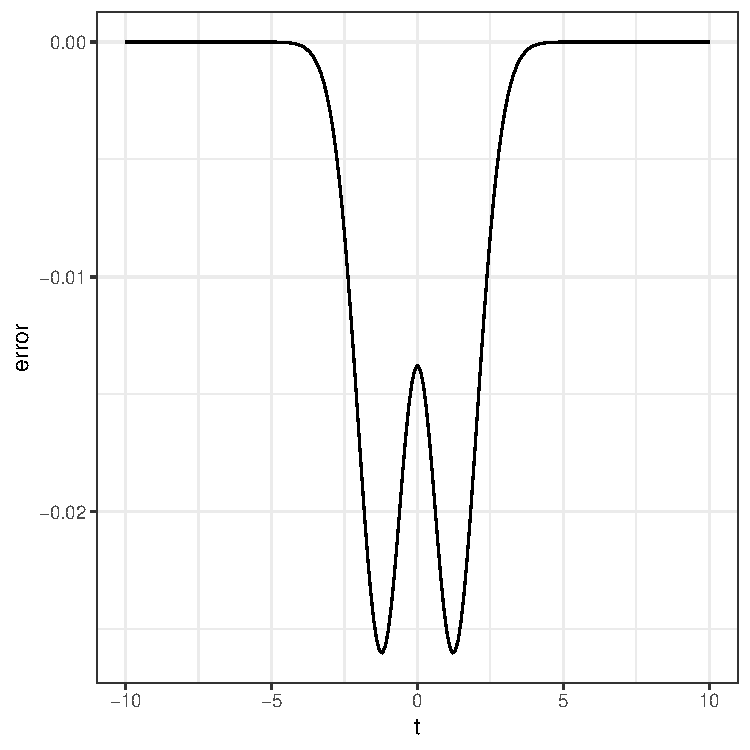
\includegraphics[width=\maxwidth]{figure/unnamed-chunk-3-1} 
\end{knitrout}
  \item Suppose we wanted to have a tail probability within 10\% of the desired
  $\alpha=0.05$. Recall we did a left-tailed test using the further data.
  How large of a sample size would we need? That is, we need
  to solve the error formula equal to 10\% of the desired left-tail probability:
  \[0.10 \alpha  \stackrel{set}{=} \underbrace{\frac{\text{skew}}{\sqrt{n}} \frac{(2t^2+1)}{6} f_Z(t)}_{\textrm{error}},\]
  which yields
  \[ n = \left(\frac{\text{skew}}{6(0.10\alpha)} (2t^2 + 1) f_Z(t)\right)^2.\]
\end{enumerate} 

  \textbf{Solution:} Below is code to find the ideal sample size.
\begin{knitrout}\scriptsize
\definecolor{shadecolor}{rgb}{0.969, 0.969, 0.969}\color{fgcolor}\begin{kframe}
\begin{alltt}
\hlcom{# Use quantile to get a specific value of t at the 5th percentile of the "further" data}
\hldef{t} \hlkwb{<-} \hlkwd{quantile}\hldef{(finches}\hlopt{$}\hldef{further,} \hlnum{0.05}\hldef{)}

\hlcom{# Calculate the sample size n based on skewness, standard deviation, and a chosen error margin (0.1) at the 5th percentile}
\hldef{n} \hlkwb{<-} \hldef{((}\hlkwd{skewness}\hldef{(finches}\hlopt{$}\hldef{further)} \hlopt{/} \hldef{(}\hlnum{6} \hlopt{*} \hlnum{0.10} \hlopt{*} \hlnum{0.05}\hldef{))} \hlopt{*} \hldef{(}\hlnum{2} \hlopt{*} \hldef{(t} \hlopt{**} \hlnum{2}\hldef{)} \hlopt{+} \hlnum{1}\hldef{)} \hlopt{*} \hlkwd{dnorm}\hldef{(t))} \hlopt{**} \hlnum{2}

\hlkwd{as.numeric}\hldef{(n)}
\end{alltt}
\begin{verbatim}
## [1] 260.6018
\end{verbatim}
\end{kframe}
\end{knitrout}
%%%%%%%%%%%%%%%%%%%%%%%%%%%%%%%%%%%%%%%%%%%%%%%%%%%%%%%%%%%%%%%%%%%%%%%%%%%%%%%%
%%%%%%%%%%%%%%%%%%%%%%%%%%%%%%%%%%%%%%%%%%%%%%%%%%%%%%%%%%%%%%%%%%%%%%%%%%%%%%%%
% Question 3
%%%%%%%%%%%%%%%%%%%%%%%%%%%%%%%%%%%%%%%%%%%%%%%%%%%%%%%%%%%%%%%%%%%%%%%%%%%%%%%%
%%%%%%%%%%%%%%%%%%%%%%%%%%%%%%%%%%%%%%%%%%%%%%%%%%%%%%%%%%%%%%%%%%%%%%%%%%%%%%%%
\item Complete the following steps to revisit the analyses from lab 11 using the
bootstrap procedure.
\begin{enumerate}
\item Now, consider the zebra finch data. We do not know the generating distributions
for the closer, further, and difference data, so perform resampling to approximate the 
sampling distribution of the $T$ statistic:
  \[T = \frac{\bar{x}_r - 0}{s/\sqrt{n}},\]
  where $\bar{x}_r$ is the mean computed on the r$^{th}$ resample and $s$ is the
  sample standard deviation from the original samples. At the end, create an
  object called \texttt{resamples.null.closer}, for example, and store the 
  resamples shifted to ensure they are consistent with the null hypotheses at the average 
  (i.e., here ensure the shifted resamples are 0 on average, corresponding
  to $t=0$, for each case). 
  
  \textbf{Solution:} Below is code to get a resampled, shifted dataset for each case in the finches data.
\begin{knitrout}\scriptsize
\definecolor{shadecolor}{rgb}{0.969, 0.969, 0.969}\color{fgcolor}\begin{kframe}
\begin{alltt}
\hlcom{# Define the number of bootstrap iterations (R)}
\hldef{R} \hlkwb{<-} \hlnum{1000}

\hlcom{# Function for bootstrapping and shifting resamples to approximate the sampling distribution}
\hldef{bootstrap.shift} \hlkwb{<-} \hlkwa{function}\hldef{(}\hlkwc{data}\hldef{,} \hlkwc{s}\hldef{,} \hlkwc{n}\hldef{,} \hlkwc{R}\hldef{) \{}
\hldef{data} \hlkwb{<-} \hldef{data} \hlopt{-} \hlkwd{mean}\hldef{(data)}
\hldef{resampled.data} \hlkwb{<-} \hlkwd{tibble}\hldef{(}\hlkwc{ts} \hldef{=} \hlkwd{rep}\hldef{(}\hlnum{NA}\hldef{, R))}  \hlcom{# Initialize a tibble to store the bootstrap t-statistics}

\hlcom{# Perform resampling R times}
\hlkwa{for}\hldef{(i} \hlkwa{in} \hlnum{1}\hlopt{:}\hldef{R) \{}
  \hldef{resamples} \hlkwb{<-} \hlkwd{sample}\hldef{(data,} \hlkwc{size} \hldef{= n,} \hlkwc{replace} \hldef{=} \hlnum{TRUE}\hldef{)}  \hlcom{# Resample with replacement}
  \hldef{resampled.data}\hlopt{$}\hldef{ts[i]} \hlkwb{<-} \hlkwd{mean}\hldef{(resamples)} \hlopt{/} \hldef{(s} \hlopt{/} \hlkwd{sqrt}\hldef{(n))}  \hlcom{# Calculate t-statistic for each resample}
\hldef{\}}

\hldef{resampled.shifted.data} \hlkwb{<-} \hlkwd{tibble}\hldef{(}\hlkwc{ts} \hldef{= resampled.data}\hlopt{$}\hldef{ts)} \hlcom{#Store data in tibble}

\hlkwd{return}\hldef{(resampled.shifted.data)}  \hlcom{# Return the shifted resample data}
\hldef{\}}

\hlcom{# Generate shifted resamples for the 'closer', 'further', and 'difference' data}
\hldef{resamples.null.closer} \hlkwb{<-} \hlkwd{bootstrap.shift}\hldef{(finches}\hlopt{$}\hldef{closer,} \hlkwc{s} \hldef{=} \hlkwd{sd}\hldef{(finches}\hlopt{$}\hldef{closer), n, R)}
\hldef{resamples.null.farther} \hlkwb{<-} \hlkwd{bootstrap.shift}\hldef{(finches}\hlopt{$}\hldef{further,} \hlkwc{s} \hldef{=} \hlkwd{sd}\hldef{(finches}\hlopt{$}\hldef{further), n, R)}
\hldef{resamples.null.diff} \hlkwb{<-} \hlkwd{bootstrap.shift}\hldef{(finches}\hlopt{$}\hldef{diff,} \hlkwc{s} \hldef{=} \hlkwd{sd}\hldef{(finches}\hlopt{$}\hldef{diff), n, R)}
\end{alltt}
\end{kframe}
\end{knitrout}
  \item Compute the bootstrap $p$-value for each test using the shifted resamples. 
  How do these compare to the $t$-test $p$-values?
  
  \textbf{Solution:} Below is code to get the bootstrapped p-values for each case of the finch data. As seen by our computed values, bootstrapped p-values and t-test p-values are practically the same.
\begin{knitrout}\scriptsize
\definecolor{shadecolor}{rgb}{0.969, 0.969, 0.969}\color{fgcolor}\begin{kframe}
\begin{alltt}
\hlcom{# Function for calculating bootstrap p-values}
\hldef{bootstrap.pval} \hlkwb{<-} \hlkwa{function}\hldef{(}\hlkwc{shifted.data}\hldef{,} \hlkwc{observed.t}\hldef{,} \hlkwc{method}\hldef{) \{}
\hlkwa{if}\hldef{(method} \hlopt{==} \hlsng{"less"}\hldef{) \{}
  \hldef{boot.pval} \hlkwb{<-} \hlkwd{mean}\hldef{(shifted.data}\hlopt{$}\hldef{ts} \hlopt{<=} \hldef{observed.t)}  \hlcom{# P-value for a "less" alternative}
\hldef{\}} \hlkwa{else if}\hldef{(method} \hlopt{==} \hlsng{"greater"}\hldef{) \{}
  \hldef{boot.pval} \hlkwb{<-} \hlkwd{mean}\hldef{(shifted.data}\hlopt{$}\hldef{ts} \hlopt{>=} \hldef{observed.t)}  \hlcom{# P-value for a "greater" alternative}
\hldef{\}} \hlkwa{else if}\hldef{(method} \hlopt{==} \hlsng{"two.sided"}\hldef{) \{}
  \hldef{boot.pval} \hlkwb{<-} \hlkwd{mean}\hldef{(}\hlkwd{abs}\hldef{(shifted.data}\hlopt{$}\hldef{ts)} \hlopt{>=} \hlkwd{abs}\hldef{(observed.t))}  \hlcom{# Two-sided test p-value}
\hldef{\}} \hlkwa{else} \hldef{\{}
  \hlkwd{stop}\hldef{(}\hlsng{"Enter a valid method."}\hldef{)}  \hlcom{# Handle invalid method input}
\hldef{\}}

\hlkwd{return}\hldef{(boot.pval)}  \hlcom{# Return the computed p-value}
\hldef{\}}

\hlcom{# Compute bootstrap p-values for each group: 'closer', 'further', and 'difference'}
\hldef{closer.pval.boot} \hlkwb{<-} \hlkwd{bootstrap.pval}\hldef{(resamples.null.closer,}
                      \hlkwc{observed.t} \hldef{=} \hlkwd{mean}\hldef{(finches}\hlopt{$}\hldef{closer)} \hlopt{/} \hldef{(}\hlkwd{sd}\hldef{(finches}\hlopt{$}\hldef{closer)} \hlopt{/} \hlkwd{sqrt}\hldef{(n)),} \hlkwc{method} \hldef{=} \hlsng{"greater"}\hldef{)}
\hldef{farther.pval.boot} \hlkwb{<-} \hlkwd{bootstrap.pval}\hldef{(resamples.null.farther,}
                      \hlkwc{observed.t} \hldef{=} \hlkwd{mean}\hldef{(finches}\hlopt{$}\hldef{further)} \hlopt{/} \hldef{(}\hlkwd{sd}\hldef{(finches}\hlopt{$}\hldef{further)} \hlopt{/} \hlkwd{sqrt}\hldef{(n)),} \hlkwc{method} \hldef{=} \hlsng{"less"}\hldef{)}
\hldef{diff.pval.boot} \hlkwb{<-} \hlkwd{bootstrap.pval}\hldef{(resamples.null.diff,}
                      \hlkwc{observed.t} \hldef{=} \hlkwd{mean}\hldef{(finches}\hlopt{$}\hldef{diff)} \hlopt{/} \hldef{(}\hlkwd{sd}\hldef{(finches}\hlopt{$}\hldef{diff)} \hlopt{/} \hlkwd{sqrt}\hldef{(n)),} \hlkwc{method} \hldef{=} \hlsng{"two.sided"}\hldef{)}

\hlcom{# Compute t-test p-values for comparison}
\hldef{closer.pval.ttest} \hlkwb{<-} \hlkwd{t.test}\hldef{(finches}\hlopt{$}\hldef{closer,} \hlkwc{mu} \hldef{=} \hlnum{0}\hldef{,} \hlkwc{alternative} \hldef{=} \hlsng{"greater"}\hldef{)}\hlopt{$}\hldef{p.value}
\hldef{farther.pval.ttest} \hlkwb{<-} \hlkwd{t.test}\hldef{(finches}\hlopt{$}\hldef{further,} \hlkwc{mu} \hldef{=} \hlnum{0}\hldef{,} \hlkwc{alternative} \hldef{=} \hlsng{"less"}\hldef{)}\hlopt{$}\hldef{p.value}
\hldef{diff.pval.ttest} \hlkwb{<-} \hlkwd{t.test}\hldef{(finches}\hlopt{$}\hldef{diff,} \hlkwc{mu} \hldef{=} \hlnum{0}\hldef{,} \hlkwc{alternative} \hldef{=} \hlsng{"two.sided"}\hldef{)}\hlopt{$}\hldef{p.value}

\hldef{closer.pval.boot}
\end{alltt}
\begin{verbatim}
## [1] 0
\end{verbatim}
\begin{alltt}
\hldef{farther.pval.boot}
\end{alltt}
\begin{verbatim}
## [1] 0
\end{verbatim}
\begin{alltt}
\hldef{diff.pval.boot}
\end{alltt}
\begin{verbatim}
## [1] 0
\end{verbatim}
\begin{alltt}
\hldef{closer.pval.ttest}
\end{alltt}
\begin{verbatim}
## [1] 8.131533e-09
\end{verbatim}
\begin{alltt}
\hldef{farther.pval.ttest}
\end{alltt}
\begin{verbatim}
## [1] 2.587359e-08
\end{verbatim}
\begin{alltt}
\hldef{diff.pval.ttest}
\end{alltt}
\begin{verbatim}
## [1] 1.036907e-08
\end{verbatim}
\end{kframe}
\end{knitrout}
    \item What is the 5$^{th}$ percentile of the shifted resamples under the null hypothesis? 
  Note this value approximates $t_{0.05, n-1}$. Compare these values in each case. 
  
  \textbf{Solution:} Below is code to get the 5$^{th}$ percentile of the shifted resamples under the null hypothesis for each case in the finch data. As seen by our computed values, our 5$^{th}$ percentiles are very similar to the approximation of $t_{0.05, n-1}$.
\begin{knitrout}\scriptsize
\definecolor{shadecolor}{rgb}{0.969, 0.969, 0.969}\color{fgcolor}\begin{kframe}
\begin{alltt}
\hlcom{# Compute the 5th percentile from the shifted resamples (bootstrap) and compare to the theoretical 5th percentile t-value}
\hldef{closer.5th} \hlkwb{<-} \hlkwd{quantile}\hldef{(resamples.null.closer}\hlopt{$}\hldef{ts,} \hlkwc{probs} \hldef{=} \hlnum{0.05}\hldef{)}
\hldef{farther.5th} \hlkwb{<-} \hlkwd{quantile}\hldef{(resamples.null.farther}\hlopt{$}\hldef{ts,} \hlkwc{probs} \hldef{=} \hlnum{0.05}\hldef{)}
\hldef{diff.5th} \hlkwb{<-} \hlkwd{quantile}\hldef{(resamples.null.diff}\hlopt{$}\hldef{ts,} \hlkwc{probs} \hldef{=} \hlnum{0.05}\hldef{)}
\hldef{t.5th} \hlkwb{<-} \hlkwd{qt}\hldef{(}\hlnum{0.05}\hldef{,} \hlkwc{df} \hldef{= n} \hlopt{-} \hlnum{1}\hldef{)}  \hlcom{# Theoretical t-value at the 5th percentile}

\hldef{closer.5th}
\end{alltt}
\begin{verbatim}
##        5% 
## -1.570544
\end{verbatim}
\begin{alltt}
\hldef{farther.5th}
\end{alltt}
\begin{verbatim}
##        5% 
## -1.688405
\end{verbatim}
\begin{alltt}
\hldef{diff.5th}
\end{alltt}
\begin{verbatim}
##        5% 
## -1.561186
\end{verbatim}
\begin{alltt}
\hldef{t.5th}
\end{alltt}
\begin{verbatim}
## [1] -1.650744
\end{verbatim}
\end{kframe}
\end{knitrout}
  \item Compute the bootstrap confidence intervals using the resamples. How do these 
  compare to the $t$-test confidence intervals? 
  
\textbf{Solution:} Below is code to get the bootstrapped confidence interval for each case in the finches data. As seen by our computed CIs, t-test CIs and bootstrapped CIs are practically identical/similar.
\begin{knitrout}\scriptsize
\definecolor{shadecolor}{rgb}{0.969, 0.969, 0.969}\color{fgcolor}\begin{kframe}
\begin{alltt}
\hlcom{# Function to compute bootstrap confidence intervals}
\hldef{bootstrap.CI} \hlkwb{<-} \hlkwa{function}\hldef{(}\hlkwc{data}\hldef{,} \hlkwc{s}\hldef{,} \hlkwc{n}\hldef{,} \hlkwc{R}\hldef{) \{}
\hldef{resampled.data} \hlkwb{<-} \hlkwd{tibble}\hldef{(}\hlkwc{ts} \hldef{=} \hlkwd{rep}\hldef{(}\hlnum{NA}\hldef{, R))}  \hlcom{# Initialize tibble to store means}

\hlcom{# Perform resampling R times}
\hlkwa{for}\hldef{(i} \hlkwa{in} \hlnum{1}\hlopt{:}\hldef{R) \{}
  \hldef{resamples} \hlkwb{<-} \hlkwd{sample}\hldef{(data,} \hlkwc{size} \hldef{= n,} \hlkwc{replace} \hldef{=} \hlnum{TRUE}\hldef{)}  \hlcom{# Resample with replacement}
  \hldef{resampled.data}\hlopt{$}\hldef{xbars[i]} \hlkwb{<-} \hlkwd{mean}\hldef{(resamples)}  \hlcom{# Store the mean of each resample}
\hldef{\}}

\hlkwd{return}\hldef{(}\hlkwd{quantile}\hldef{(resampled.data}\hlopt{$}\hldef{xbars,} \hlkwd{c}\hldef{(}\hlnum{0.025}\hldef{,} \hlnum{0.975}\hldef{)))}  \hlcom{# Return 95% confidence interval using percentiles}
\hldef{\}}

\hlcom{# Compute bootstrap confidence intervals for the three datasets}
\hldef{boot.CI.closer} \hlkwb{<-} \hlkwd{bootstrap.CI}\hldef{(finches}\hlopt{$}\hldef{closer,} \hlkwc{s} \hldef{=} \hlkwd{sd}\hldef{(finches}\hlopt{$}\hldef{closer), n, R)}
\hldef{boot.CI.farther} \hlkwb{<-} \hlkwd{bootstrap.CI}\hldef{(finches}\hlopt{$}\hldef{further,} \hlkwc{s} \hldef{=} \hlkwd{sd}\hldef{(finches}\hlopt{$}\hldef{further), n, R)}
\hldef{boot.CI.diff} \hlkwb{<-} \hlkwd{bootstrap.CI}\hldef{(finches}\hlopt{$}\hldef{diff,} \hlkwc{s} \hldef{=} \hlkwd{sd}\hldef{(finches}\hlopt{$}\hldef{diff), n, R)}

\hlcom{# Compute t-test confidence intervals for comparison}
\hldef{ttest.CI.closer} \hlkwb{<-} \hlkwd{t.test}\hldef{(finches}\hlopt{$}\hldef{closer,} \hlkwc{mu} \hldef{=} \hlnum{0}\hldef{,} \hlkwc{alternative} \hldef{=} \hlsng{"two.sided"}\hldef{)}\hlopt{$}\hldef{conf.int}
\hldef{ttest.CI.farther} \hlkwb{<-} \hlkwd{t.test}\hldef{(finches}\hlopt{$}\hldef{further,} \hlkwc{mu} \hldef{=} \hlnum{0}\hldef{,} \hlkwc{alternative} \hldef{=} \hlsng{"two.sided"}\hldef{)}\hlopt{$}\hldef{conf.int}
\hldef{ttest.CI.diff} \hlkwb{<-} \hlkwd{t.test}\hldef{(finches}\hlopt{$}\hldef{diff,} \hlkwc{mu} \hldef{=} \hlnum{0}\hldef{,} \hlkwc{alternative} \hldef{=} \hlsng{"two.sided"}\hldef{)}\hlopt{$}\hldef{conf.int}

\hldef{boot.CI.closer}
\end{alltt}
\begin{verbatim}
##      2.5%     97.5% 
## 0.1452800 0.1672061
\end{verbatim}
\begin{alltt}
\hldef{boot.CI.farther}
\end{alltt}
\begin{verbatim}
##       2.5%      97.5% 
## -0.2184547 -0.1875324
\end{verbatim}
\begin{alltt}
\hldef{boot.CI.diff}
\end{alltt}
\begin{verbatim}
##      2.5%     97.5% 
## 0.3341395 0.3835500
\end{verbatim}
\begin{alltt}
\hldef{ttest.CI.closer}
\end{alltt}
\begin{verbatim}
## [1] 0.1173875 0.1950586
## attr(,"conf.level")
## [1] 0.95
\end{verbatim}
\begin{alltt}
\hldef{ttest.CI.farther}
\end{alltt}
\begin{verbatim}
## [1] -0.2565176 -0.1489313
## attr(,"conf.level")
## [1] 0.95
\end{verbatim}
\begin{alltt}
\hldef{ttest.CI.diff}
\end{alltt}
\begin{verbatim}
## [1] 0.2719028 0.4459921
## attr(,"conf.level")
## [1] 0.95
\end{verbatim}
\end{kframe}
\end{knitrout}
\end{enumerate}
%%%%%%%%%%%%%%%%%%%%%%%%%%%%%%%%%%%%%%%%%%%%%%%%%%%%%%%%%%%%%%%%%%%%%%%%%%%%%%%%
%%%%%%%%%%%%%%%%%%%%%%%%%%%%%%%%%%%%%%%%%%%%%%%%%%%%%%%%%%%%%%%%%%%%%%%%%%%%%%%%
% Question 4
%%%%%%%%%%%%%%%%%%%%%%%%%%%%%%%%%%%%%%%%%%%%%%%%%%%%%%%%%%%%%%%%%%%%%%%%%%%%%%%%
%%%%%%%%%%%%%%%%%%%%%%%%%%%%%%%%%%%%%%%%%%%%%%%%%%%%%%%%%%%%%%%%%%%%%%%%%%%%%%%%
\item Complete the following steps to revisit the analyses from lab 11 using the
randomization procedure.
\begin{enumerate}
\item Now, consider the zebra finch data. We do not know the generating distributions
for the closer, further, and difference data, so perform the randomization procedure 

\textbf{Solution:} Below is code to perform the randomization procedure for each case in the finch data.
\begin{knitrout}\scriptsize
\definecolor{shadecolor}{rgb}{0.969, 0.969, 0.969}\color{fgcolor}\begin{kframe}
\begin{alltt}
\hldef{random.data} \hlkwb{<-} \hlkwa{function}\hldef{(}\hlkwc{data}\hldef{,} \hlkwc{mu0}\hldef{,} \hlkwc{R} \hldef{=} \hlnum{1000}\hldef{) \{}
  \hldef{rand} \hlkwb{<-} \hlkwd{tibble}\hldef{(}\hlkwc{means} \hldef{=} \hlkwd{rep}\hldef{(}\hlnum{NA}\hldef{, R))}  \hlcom{# Initialize tibble to store means}

  \hldef{x.shift} \hlkwb{<-} \hldef{data} \hlopt{-} \hldef{mu0}  \hlcom{# Shift the data by subtracting the hypothesized mean}

  \hlkwa{for}\hldef{(i} \hlkwa{in} \hlnum{1}\hlopt{:}\hldef{R) \{}
    \hldef{curr.rand} \hlkwb{<-} \hldef{x.shift} \hlopt{*} \hlkwd{sample}\hldef{(}\hlkwc{x} \hldef{=} \hlkwd{c}\hldef{(}\hlopt{-}\hlnum{1}\hldef{,} \hlnum{1}\hldef{),} \hlkwc{size} \hldef{=} \hlkwd{length}\hldef{(x.shift),} \hlkwc{replace} \hldef{=} \hlnum{TRUE}\hldef{)}  \hlcom{# Randomize the signs}
    \hldef{rand}\hlopt{$}\hldef{means[i]} \hlkwb{<-} \hlkwd{mean}\hldef{(curr.rand)}  \hlcom{# Store the mean of each randomization}
  \hldef{\}}

  \hlkwd{return}\hldef{(rand)}
\hldef{\}}

\hldef{closer.rand} \hlkwb{<-} \hlkwd{random.data}\hldef{(finches}\hlopt{$}\hldef{closer,} \hlnum{0}\hldef{)}
\hldef{farther.rand} \hlkwb{<-} \hlkwd{random.data}\hldef{(finches}\hlopt{$}\hldef{further,} \hlnum{0}\hldef{)}
\hldef{diff.rand} \hlkwb{<-} \hlkwd{random.data}\hldef{(finches}\hlopt{$}\hldef{diff,} \hlnum{0}\hldef{)}
\end{alltt}
\end{kframe}
\end{knitrout}
  \item Compute the randomization test $p$-value for each test. 
  
\textbf{Solution:} Below is code to get the randomized p-value for each case in the finch data.
\begin{knitrout}\scriptsize
\definecolor{shadecolor}{rgb}{0.969, 0.969, 0.969}\color{fgcolor}\begin{kframe}
\begin{alltt}
\hlcom{# Randomization procedure to compute p-values and confidence intervals for a random hypothesis test}
\hldef{random.pval} \hlkwb{<-} \hlkwa{function}\hldef{(}\hlkwc{data}\hldef{,} \hlkwc{mu0}\hldef{,} \hlkwc{method} \hldef{=} \hlsng{"two.sided"}\hldef{,} \hlkwc{R} \hldef{=} \hlnum{1000}\hldef{) \{}
\hldef{rand} \hlkwb{<-} \hlkwd{tibble}\hldef{(}\hlkwc{means} \hldef{=} \hlkwd{rep}\hldef{(}\hlnum{NA}\hldef{, R))}  \hlcom{# Initialize tibble to store means}

\hldef{x.shift} \hlkwb{<-} \hldef{data} \hlopt{-} \hldef{mu0}  \hlcom{# Shift the data by subtracting the hypothesized mean}

\hlkwa{for}\hldef{(i} \hlkwa{in} \hlnum{1}\hlopt{:}\hldef{R) \{}
  \hldef{curr.rand} \hlkwb{<-} \hldef{x.shift} \hlopt{*} \hlkwd{sample}\hldef{(}\hlkwc{x} \hldef{=} \hlkwd{c}\hldef{(}\hlopt{-}\hlnum{1}\hldef{,} \hlnum{1}\hldef{),} \hlkwc{size} \hldef{=} \hlkwd{length}\hldef{(x.shift),} \hlkwc{replace} \hldef{=} \hlnum{TRUE}\hldef{)}  \hlcom{# Randomize the signs}
  \hldef{rand}\hlopt{$}\hldef{means[i]} \hlkwb{<-} \hlkwd{mean}\hldef{(curr.rand)}  \hlcom{# Store the mean of each randomization}
\hldef{\}}

\hldef{delta} \hlkwb{<-} \hlkwd{abs}\hldef{(}\hlkwd{mean}\hldef{(data))}  \hlcom{# Calculate the difference from the hypothesized mean}
\hldef{low} \hlkwb{<-} \hlnum{0} \hlopt{-} \hldef{delta}  \hlcom{# Lower bound for the CI}
\hldef{high} \hlkwb{<-} \hlnum{0} \hlopt{+} \hldef{delta}  \hlcom{# Upper bound for the CI}

\hlcom{# Compute p-values based on the randomization}
\hlkwa{if}\hldef{(method} \hlopt{==} \hlsng{"less"}\hldef{) \{}
  \hlkwd{return}\hldef{(}\hlkwd{mean}\hldef{(rand}\hlopt{$}\hldef{means} \hlopt{<=} \hldef{low))}
\hldef{\}} \hlkwa{else if}\hldef{(method} \hlopt{==} \hlsng{"greater"}\hldef{) \{}
  \hlkwd{return}\hldef{(}\hlkwd{mean}\hldef{(rand}\hlopt{$}\hldef{means} \hlopt{>=} \hldef{high))}
\hldef{\}} \hlkwa{else if}\hldef{(method} \hlopt{==} \hlsng{"two.sided"}\hldef{) \{}
  \hlkwd{return}\hldef{(}\hlkwd{mean}\hldef{(rand}\hlopt{$}\hldef{means} \hlopt{<=} \hldef{low)} \hlopt{+} \hlkwd{mean}\hldef{(rand}\hlopt{$}\hldef{means} \hlopt{>=} \hldef{high))}
\hldef{\}} \hlkwa{else} \hldef{\{}
  \hlkwd{stop}\hldef{(}\hlsng{"Enter a valid method."}\hldef{)}  \hlcom{# Handle invalid method input}
\hldef{\}}
\hldef{\}}

\hlcom{# Compute random p-values for each group}
\hldef{closer.rand.pval} \hlkwb{<-} \hlkwd{random.pval}\hldef{(finches}\hlopt{$}\hldef{closer,} \hlnum{0}\hldef{,} \hlsng{"greater"}\hldef{)}
\hldef{farther.rand.pval} \hlkwb{<-} \hlkwd{random.pval}\hldef{(finches}\hlopt{$}\hldef{further,} \hlnum{0}\hldef{,} \hlsng{"less"}\hldef{)}
\hldef{diff.rand.pval} \hlkwb{<-} \hlkwd{random.pval}\hldef{(finches}\hlopt{$}\hldef{diff,} \hlnum{0}\hldef{)}

\hldef{closer.rand.pval}
\end{alltt}
\begin{verbatim}
## [1] 0
\end{verbatim}
\begin{alltt}
\hldef{farther.rand.pval}
\end{alltt}
\begin{verbatim}
## [1] 0
\end{verbatim}
\begin{alltt}
\hldef{diff.rand.pval}
\end{alltt}
\begin{verbatim}
## [1] 0
\end{verbatim}
\end{kframe}
\end{knitrout}
  \item Compute the randomization confidence interval by iterating over values of $\mu_0$.
  
\textbf{Solution:} Below is code to get the randomized confidence intervals for each case in the finch data.
\begin{knitrout}\scriptsize
\definecolor{shadecolor}{rgb}{0.969, 0.969, 0.969}\color{fgcolor}\begin{kframe}
\begin{alltt}
\hlcom{# Randomized Confidence Interval procedure}
\hldef{random.CI} \hlkwb{<-} \hlkwa{function}\hldef{(}\hlkwc{data}\hldef{,}
                    \hlkwc{R} \hldef{=} \hlnum{1000}\hldef{)\{}
\hldef{mu0.iterate} \hlkwb{<-} \hlnum{0.01} \hlcom{#Iteration Variable}
\hldef{starting.point} \hlkwb{<-} \hlkwd{mean}\hldef{(data)} \hlcom{#Starting Point}
\hldef{mu.lower} \hlkwb{<-} \hldef{starting.point} \hlcom{# Initialize lower bound for CI}

\hlkwa{repeat}\hldef{\{}
  \hldef{rand} \hlkwb{<-} \hlkwd{tibble}\hldef{(}\hlkwc{means} \hldef{=} \hlkwd{rep}\hldef{(}\hlnum{NA}\hldef{, R))} \hlcom{# Initialize tibble for storing means}
  \hldef{x.shift} \hlkwb{<-} \hldef{data} \hlopt{-} \hldef{mu.lower} \hlcom{# Shift data}

  \hlkwa{for}\hldef{(i} \hlkwa{in} \hlnum{1}\hlopt{:}\hldef{R)\{}
    \hldef{curr.rand} \hlkwb{<-} \hldef{x.shift} \hlopt{*} \hlcom{# Randomize the data}
      \hlkwd{sample}\hldef{(}\hlkwc{x} \hldef{=} \hlkwd{c}\hldef{(}\hlopt{-}\hlnum{1}\hldef{,}\hlnum{1}\hldef{),}
             \hlkwc{size} \hldef{=} \hlkwd{length}\hldef{(x.shift),}
             \hlkwc{replace} \hldef{=} \hlnum{TRUE}\hldef{)}

    \hldef{rand}\hlopt{$}\hldef{means[i]} \hlkwb{<-} \hlkwd{mean}\hldef{(curr.rand)} \hlcom{# Store mean of each randomization}
  \hldef{\}}

  \hldef{delta} \hlkwb{<-} \hlkwd{abs}\hldef{(}\hlkwd{mean}\hldef{(data))} \hlcom{# Calculate delta from the me}
  \hldef{low} \hlkwb{<-} \hlnum{0} \hlopt{-} \hldef{delta} \hlcom{# Lower bound for CI}
  \hldef{high}\hlkwb{<-} \hlnum{0} \hlopt{+} \hldef{delta} \hlcom{# Upper bound for CI}

  \hldef{rand} \hlkwb{<-} \hldef{rand |>}
    \hlkwd{mutate}\hldef{(}\hlkwc{means} \hldef{= means} \hlopt{+} \hldef{mu.lower)} \hlcom{# Compute p-value}
  \hldef{delta} \hlkwb{<-} \hlkwd{abs}\hldef{(}\hlkwd{mean}\hldef{(data)} \hlopt{-} \hldef{mu.lower)}
  \hldef{low} \hlkwb{<-} \hldef{mu.lower} \hlopt{-} \hldef{delta}
  \hldef{high}\hlkwb{<-} \hldef{mu.lower} \hlopt{+} \hldef{delta}
  \hldef{p.val} \hlkwb{<-} \hlkwd{mean}\hldef{(rand}\hlopt{$}\hldef{means} \hlopt{<=} \hldef{low)} \hlopt{+}
    \hlkwd{mean}\hldef{(rand}\hlopt{$}\hldef{means} \hlopt{>=} \hldef{high)}

  \hlkwa{if}\hldef{(p.val} \hlopt{<} \hlnum{0.05}\hldef{)\{} \hlcom{# Stop if p-value is less than 0.05}
    \hlkwa{break}
  \hldef{\}}\hlkwa{else}\hldef{\{}
    \hldef{mu.lower} \hlkwb{<-} \hldef{mu.lower} \hlopt{-} \hldef{mu0.iterate} \hlcom{# Otherwise, shift lower bound further}
  \hldef{\}}
\hldef{\}}

\hldef{mu0.iterate} \hlkwb{<-} \hlnum{0.01}  \hlcom{# Repeat for upper bound}
\hldef{starting.point} \hlkwb{<-} \hlkwd{mean}\hldef{(data)}
\hldef{mu.higher} \hlkwb{<-} \hldef{starting.point}

\hlkwa{repeat}\hldef{\{}
  \hldef{rand} \hlkwb{<-} \hlkwd{tibble}\hldef{(}\hlkwc{means} \hldef{=} \hlkwd{rep}\hldef{(}\hlnum{NA}\hldef{, R))}
  \hldef{x.shift} \hlkwb{<-} \hldef{data} \hlopt{-} \hldef{mu.higher}

  \hlkwa{for}\hldef{(i} \hlkwa{in} \hlnum{1}\hlopt{:}\hldef{R)\{}
    \hldef{curr.rand} \hlkwb{<-} \hldef{x.shift} \hlopt{*}
      \hlkwd{sample}\hldef{(}\hlkwc{x} \hldef{=} \hlkwd{c}\hldef{(}\hlopt{-}\hlnum{1}\hldef{,}\hlnum{1}\hldef{),}
             \hlkwc{size} \hldef{=} \hlkwd{length}\hldef{(x.shift),}
             \hlkwc{replace} \hldef{=} \hlnum{TRUE}\hldef{)}

    \hldef{rand}\hlopt{$}\hldef{means[i]} \hlkwb{<-} \hlkwd{mean}\hldef{(curr.rand)}
  \hldef{\}}

  \hldef{delta} \hlkwb{<-} \hlkwd{abs}\hldef{(}\hlkwd{mean}\hldef{(data))}
  \hldef{high} \hlkwb{<-} \hlnum{0} \hlopt{+} \hldef{delta}

  \hldef{rand} \hlkwb{<-} \hldef{rand |>}
    \hlkwd{mutate}\hldef{(}\hlkwc{means} \hldef{= means} \hlopt{+} \hldef{mu.higher)}
  \hldef{delta} \hlkwb{<-} \hlkwd{abs}\hldef{(}\hlkwd{mean}\hldef{(data)} \hlopt{-} \hldef{mu.higher)}
  \hldef{low} \hlkwb{<-} \hldef{mu.higher} \hlopt{-} \hldef{delta}
  \hldef{high}\hlkwb{<-} \hldef{mu.higher} \hlopt{+} \hldef{delta}
  \hldef{p.val} \hlkwb{<-} \hlkwd{mean}\hldef{(rand}\hlopt{$}\hldef{means} \hlopt{<=} \hldef{low)} \hlopt{+}
    \hlkwd{mean}\hldef{(rand}\hlopt{$}\hldef{means} \hlopt{>=} \hldef{high)}

  \hlkwa{if}\hldef{(p.val} \hlopt{<} \hlnum{0.05}\hldef{)\{}
    \hlkwa{break}
  \hldef{\}}\hlkwa{else}\hldef{\{}
    \hldef{mu.higher} \hlkwb{<-} \hldef{mu.higher} \hlopt{+} \hldef{mu0.iterate} \hlcom{# Shift upper bound higher}
  \hldef{\}}
\hldef{\}}

\hlkwd{return}\hldef{(}\hlkwd{c}\hldef{(mu.lower, mu.higher))}
\hldef{\}}

\hlcom{# Compute random confidence intervals for each group}
\hldef{closer.rand.CI} \hlkwb{<-} \hlkwd{random.CI}\hldef{(finches}\hlopt{$}\hldef{closer)}
\hldef{farther.rand.CI} \hlkwb{<-} \hlkwd{random.CI}\hldef{(finches}\hlopt{$}\hldef{further)}
\hldef{diff.rand.CI} \hlkwb{<-} \hlkwd{random.CI}\hldef{(finches}\hlopt{$}\hldef{diff)}

\hldef{closer.rand.CI}
\end{alltt}
\begin{verbatim}
## [1] 0.1162231 0.1962231
\end{verbatim}
\begin{alltt}
\hldef{farther.rand.CI}
\end{alltt}
\begin{verbatim}
## [1] -0.2627244 -0.1427244
\end{verbatim}
\begin{alltt}
\hldef{diff.rand.CI}
\end{alltt}
\begin{verbatim}
## [1] 0.2689475 0.4489475
\end{verbatim}
\end{kframe}
\end{knitrout}
  \textbf{Hint:} You can ``search" for the lower bound from $Q_1$ and subtracting by 0.0001, 
  and the upper bound using $Q_3$ and increasing by 0.0001. You will continue until you find 
  the first value for which the two-sided $p$-value is greater than or equal to 0.05.
\end{enumerate}
%%%%%%%%%%%%%%%%%%%%%%%%%%%%%%%%%%%%%%%%%%%%%%%%%%%%%%%%%%%%%%%%%%%%%%%%%%%%%%%%
%%%%%%%%%%%%%%%%%%%%%%%%%%%%%%%%%%%%%%%%%%%%%%%%%%%%%%%%%%%%%%%%%%%%%%%%%%%%%%%%
% Optional Question
%%%%%%%%%%%%%%%%%%%%%%%%%%%%%%%%%%%%%%%%%%%%%%%%%%%%%%%%%%%%%%%%%%%%%%%%%%%%%%%%
%%%%%%%%%%%%%%%%%%%%%%%%%%%%%%%%%%%%%%%%%%%%%%%%%%%%%%%%%%%%%%%%%%%%%%%%%%%%%%%%
\item \textbf{Optional Challenge:} In this lab, you performed resampling to 
approximate the sampling distribution of the $T$ statistic using
\[T = \frac{\bar{x}_r - 0}{s/\sqrt{n}}.\]
I'm curious whether it is better/worse/similar if we computed the statistics
using the sample standard deviation of the resamples ($s_r$), instead of the 
original sample ($s$)
  \[T = \frac{\bar{x}_r - 0}{s_r/\sqrt{n}}.\]
\begin{enumerate}
  \item Perform a simulation study to evaluate the Type I error for conducting this
hypothesis test both ways.

\textbf{Solution:} The code below calculates the Type I error rate for both hypothesis tests using bootstrapping techniques. As seen by our values for $s$ (\verb|type_I_error_rate_s|) and $s_r$  (\verb|type_I_error_rate_sr|), utilizing the sample standard deviation of the samples rather than the original sample inflates our Type I error rate.
\begin{knitrout}\scriptsize
\definecolor{shadecolor}{rgb}{0.969, 0.969, 0.969}\color{fgcolor}\begin{kframe}
\begin{alltt}
\hlcom{# Parameters}
\hldef{R} \hlkwb{<-} \hlnum{1000}  \hlcom{# Number of simulations}
\hldef{n} \hlkwb{=} \hlnum{30} \hlcom{# Sample size}

\hlcom{# Set up the results storage}
\hldef{simulation.dat} \hlkwb{<-} \hlkwd{tibble}\hldef{(}
  \hlkwc{sample.s.reject} \hldef{=} \hlkwd{rep}\hldef{(}\hlnum{NA}\hldef{, R),}
  \hlkwc{sample.sr.reject} \hldef{=} \hlkwd{rep}\hldef{(}\hlnum{NA}\hldef{, R)}
\hldef{)}

\hlkwa{for}\hldef{(k} \hlkwa{in} \hlnum{1}\hlopt{:}\hldef{R) \{}
  \hldef{sim.dat} \hlkwb{<-} \hlkwd{rlaplace}\hldef{(}\hlkwc{n} \hldef{= n,} \hlkwc{location} \hldef{=} \hlnum{0}\hldef{,} \hlkwc{scale} \hldef{=} \hlnum{4}\hldef{)} \hlcom{#simulate rlapace data for n = 30}
  \hldef{sim.dat.null} \hlkwb{<-} \hldef{sim.dat} \hlopt{-} \hlkwd{mean}\hldef{(sim.dat)} \hlcom{#Shift the data to null}
  \hldef{s} \hlkwb{<-} \hlkwd{sd}\hldef{(sim.dat)}
  \hldef{resample.dat} \hlkwb{<-} \hlkwd{tibble}\hldef{(}
    \hlkwc{sample.s.ts} \hldef{=} \hlkwd{rep}\hldef{(}\hlnum{NA}\hldef{, R),}
    \hlkwc{sample.sr.ts} \hldef{=} \hlkwd{rep}\hldef{(}\hlnum{NA}\hldef{, R)}
  \hldef{)}

  \hlcom{# Resampling loop}
  \hlkwa{for}\hldef{(i} \hlkwa{in} \hlnum{1}\hlopt{:}\hldef{R) \{}
    \hldef{resamples} \hlkwb{<-} \hlkwd{sample}\hldef{(sim.dat.null,} \hlkwc{size} \hldef{= n,} \hlkwc{replace} \hldef{=} \hlnum{TRUE}\hldef{)} \hlcom{# Take resamples}
    \hldef{xbar} \hlkwb{<-} \hlkwd{mean}\hldef{(resamples)}

    \hlcom{# Calculate test statistics}
    \hldef{resample.dat}\hlopt{$}\hldef{sample.s.ts[i]} \hlkwb{<-} \hldef{xbar} \hlopt{/} \hldef{(s} \hlopt{/} \hlkwd{sqrt}\hldef{(n))}  \hlcom{# Using original standard deviation}
    \hldef{resample.dat}\hlopt{$}\hldef{sample.sr.ts[i]} \hlkwb{<-} \hldef{xbar} \hlopt{/} \hldef{(}\hlkwd{sd}\hldef{(resamples)} \hlopt{/} \hlkwd{sqrt}\hldef{(n))}  \hlcom{# Using resampled standard deviation}
  \hldef{\}}

  \hlcom{# Observed t-statistic based on centered data}
  \hldef{observed.t} \hlkwb{<-} \hlkwd{mean}\hldef{(sim.dat)} \hlopt{/} \hldef{(}\hlkwd{sd}\hldef{(sim.dat)} \hlopt{/} \hlkwd{sqrt}\hldef{(n))}  \hlcom{# Corrected t-statistic}

  \hlcom{# Two-tailed p-value calculation}
  \hldef{pval.s} \hlkwb{<-} \hlkwd{mean}\hldef{(resample.dat}\hlopt{$}\hldef{sample.s.ts} \hlopt{>=} \hldef{observed.t)}  \hlcom{# For original sample SD}
  \hldef{pval.sr} \hlkwb{<-} \hlkwd{mean}\hldef{(resample.dat}\hlopt{$}\hldef{sample.sr.ts} \hlopt{>=} \hldef{observed.t)}  \hlcom{# For resampled SD}

  \hlcom{# Rejection decision based on two-tailed test}
  \hlkwa{if}\hldef{(pval.s} \hlopt{<} \hlnum{0.05}\hldef{) \{}
    \hldef{simulation.dat}\hlopt{$}\hldef{sample.s.reject[k]} \hlkwb{<-} \hlnum{1}
  \hldef{\}} \hlkwa{else} \hldef{\{}
    \hldef{simulation.dat}\hlopt{$}\hldef{sample.s.reject[k]} \hlkwb{<-} \hlnum{0}
  \hldef{\}}

  \hlkwa{if}\hldef{(pval.sr} \hlopt{<} \hlnum{0.05}\hldef{) \{}
    \hldef{simulation.dat}\hlopt{$}\hldef{sample.sr.reject[k]} \hlkwb{<-} \hlnum{1}
  \hldef{\}} \hlkwa{else} \hldef{\{}
    \hldef{simulation.dat}\hlopt{$}\hldef{sample.sr.reject[k]} \hlkwb{<-} \hlnum{0}
  \hldef{\}}
\hldef{\}}

\hlcom{# Summarize Type I error rates}
\hldef{type_I_error_rate_s} \hlkwb{<-} \hlkwd{mean}\hldef{(simulation.dat}\hlopt{$}\hldef{sample.s.reject)}
\hldef{type_I_error_rate_sr} \hlkwb{<-} \hlkwd{mean}\hldef{(simulation.dat}\hlopt{$}\hldef{sample.sr.reject)}

\hldef{type_I_error_rate_s}
\end{alltt}
\begin{verbatim}
## [1] 0.064
\end{verbatim}
\begin{alltt}
\hldef{type_I_error_rate_sr}
\end{alltt}
\begin{verbatim}
## [1] 0.07
\end{verbatim}
\end{kframe}
\end{knitrout}

  \item Using the same test case(s) as part (a), compute bootstrap confidence 
  intervals and assess their coverage -- how often do we `capture' the parameter
of interest?

\textbf{Solution:} As seen by this bootstrap CI simulation, we capture the parameter of interest $94.5\%$ of the time.
\begin{knitrout}\scriptsize
\definecolor{shadecolor}{rgb}{0.969, 0.969, 0.969}\color{fgcolor}\begin{kframe}
\begin{alltt}
\hlcom{#Store capture results}
\hldef{simulation.mean.dat} \hlkwb{<-} \hlkwd{tibble}\hldef{(}
  \hlkwc{sample.capture} \hldef{=} \hlkwd{rep}\hldef{(}\hlnum{NA}\hldef{, R)}
\hldef{)}

\hlkwa{for}\hldef{(i} \hlkwa{in} \hlnum{1}\hlopt{:}\hldef{R) \{}
  \hldef{sim.dat} \hlkwb{<-} \hlkwd{rlaplace}\hldef{(}\hlkwc{n} \hldef{= n,} \hlkwc{location} \hldef{=} \hlnum{0}\hldef{,} \hlkwc{scale} \hldef{=} \hlnum{4}\hldef{)} \hlcom{#simulate rlapace data for n = 30}
  \hldef{mu0} \hlkwb{<-} \hlkwd{mean}\hldef{(sim.dat)} \hlcom{#original mean}
  \hldef{sim.dat.null} \hlkwb{<-} \hldef{sim.dat} \hlopt{-} \hlkwd{mean}\hldef{(sim.dat)} \hlcom{#Shift the data to null}
  \hldef{resample.dats} \hlkwb{<-} \hlkwd{tibble}\hldef{(}
    \hlkwc{xbars} \hldef{=} \hlkwd{rep}\hldef{(}\hlnum{NA}\hldef{, R)}
  \hldef{)}

  \hlcom{# Resampling loop}
  \hlkwa{for}\hldef{(k} \hlkwa{in} \hlnum{1}\hlopt{:}\hldef{R) \{}
    \hldef{resamples} \hlkwb{<-} \hlkwd{sample}\hldef{(sim.dat.null,} \hlkwc{size} \hldef{= n,} \hlkwc{replace} \hldef{=} \hlnum{TRUE}\hldef{)} \hlcom{# Take resamples}
    \hldef{resample.dats}\hlopt{$}\hldef{xbars[k]} \hlkwb{<-} \hlkwd{mean}\hldef{(resamples)}
  \hldef{\}}

  \hlcom{#Compute confidence interval }
  \hldef{ci} \hlkwb{<-} \hlkwd{quantile}\hldef{(resample.dats}\hlopt{$}\hldef{xbars,} \hlkwd{c}\hldef{(}\hlnum{0.025}\hldef{,} \hlnum{0.975}\hldef{))}

  \hlcom{#Check for coverage}
  \hlkwa{if}\hldef{((mu0} \hlopt{>=} \hldef{ci[}\hlnum{1}\hldef{]} \hlopt{&&} \hldef{mu0} \hlopt{<=} \hldef{ci[}\hlnum{2}\hldef{]))\{}
    \hldef{simulation.mean.dat}\hlopt{$}\hldef{sample.capture[i]} \hlkwb{<-} \hlnum{1}
  \hldef{\}} \hlkwa{else}\hldef{\{}
    \hldef{simulation.mean.dat}\hlopt{$}\hldef{sample.capture[i]} \hlkwb{<-} \hlnum{0}
  \hldef{\}}
\hldef{\}}

\hlcom{#Calculate the capture rate}
\hldef{capture.porportion} \hlkwb{<-} \hlkwd{mean}\hldef{(simulation.mean.dat}\hlopt{$}\hldef{sample.capture)}

\hldef{capture.porportion}
\end{alltt}
\begin{verbatim}
## [1] 0.944
\end{verbatim}
\end{kframe}
\end{knitrout}

\end{enumerate}
%%%%%%%%%%%%%%%%%%%%%%%%%%%%%%%%%%%%%%%%%%%%%%%%%%%%%%%%%%%%%%%%%%%%%%%%%%%%%%%%
%%%%%%%%%%%%%%%%%%%%%%%%%%%%%%%%%%%%%%%%%%%%%%%%%%%%%%%%%%%%%%%%%%%%%%%%%%%%%%%%
% End Document
%%%%%%%%%%%%%%%%%%%%%%%%%%%%%%%%%%%%%%%%%%%%%%%%%%%%%%%%%%%%%%%%%%%%%%%%%%%%%%%%
%%%%%%%%%%%%%%%%%%%%%%%%%%%%%%%%%%%%%%%%%%%%%%%%%%%%%%%%%%%%%%%%%%%%%%%%%%%%%%%%
\end{enumerate}
\bibliography{bibliography}
\end{document}

